\subsection{Lab11: Transmisor FM Mono}

%*********************
\begin{frame}{}

\pgfdeclareimage[width=\paperwidth,height=\paperheight]{bg}{imagenes/fondo_lab}
\setbeamertemplate{background}{\pgfuseimage{bg}}

\bfseries{\textrm{\LARGE Lab11\\ \Large Transmisor FM Monofónico}}
\raggedright
\end{frame}
%*********************

\begin{frame}{Transmisor FM Monofónico}

\pgfdeclareimage[width=\paperwidth,height=\paperheight]{bg}{imagenes/fondo3}
\setbeamertemplate{background}{\pgfuseimage{bg}}

El transmisor FM es un dispositivo electrónico que, mediante una antena, irradia ondas electromagnéticas que contienen (o pueden contener) información, como ocurre en el caso de las señales de radio, televisión, telefonía móvil o cualquier otro tipo de radiocomunicación.\\
\vspace{2mm}
Por medio de la modulación angular se puede hacer que un parámetro de la onda portadora cambie de valor según las variaciones de la señal moduladora, que es la información que se quiere transmitir. \\
\vspace{2mm}
Se utiliza esta modulación porque facilita la propagación de la señal de información, ordena el radio-espectro, disminuye dimensiones de antenas, optimiza el ancho de banda de cada canal, evita interferencias entre canales, y Protege la información de las degradaciones por ruido.


\end{frame}
%---------------------------------
\begin{frame}{Transmisor FM Monofónico}

\begin{figure}[H]
\centering
\vspace{-3mm}
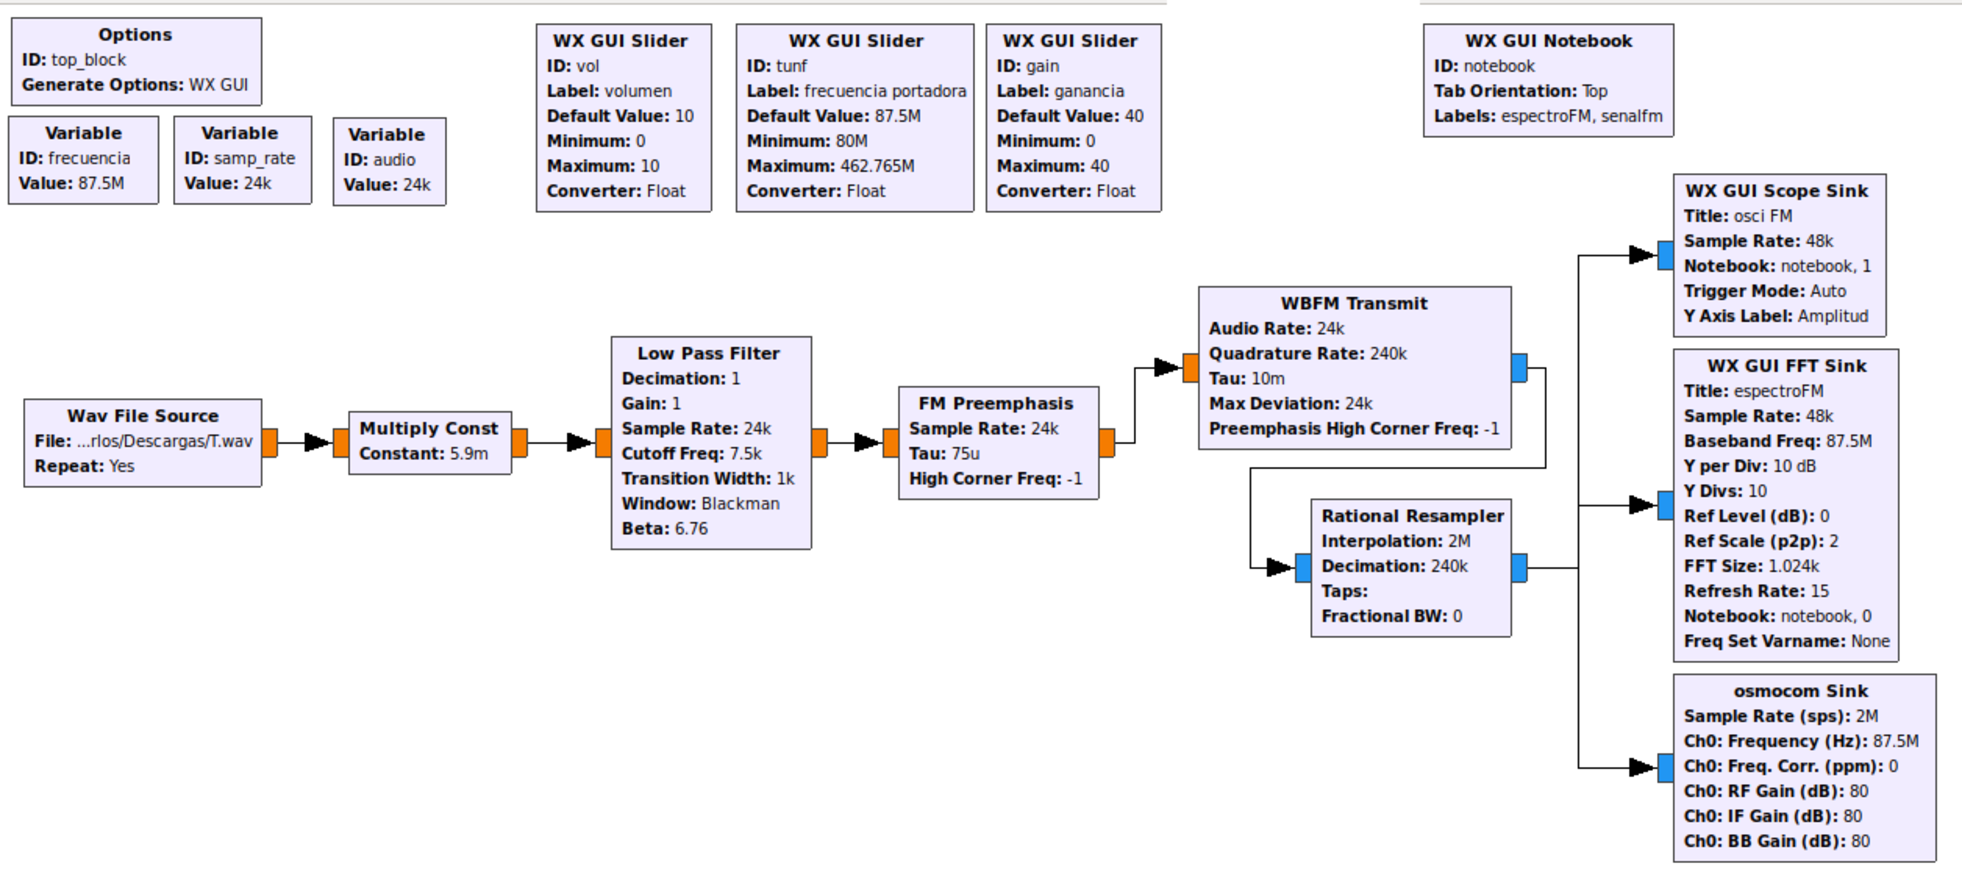
\includegraphics[width=\textwidth]{parte3/lab11/pdf/lab11_1.pdf}
\end{figure}

\end{frame}
%---------------------------------

\begin{frame}{Transmisor FM Monofónico}

\begin{figure}[H]
\centering
\vspace{-3mm}
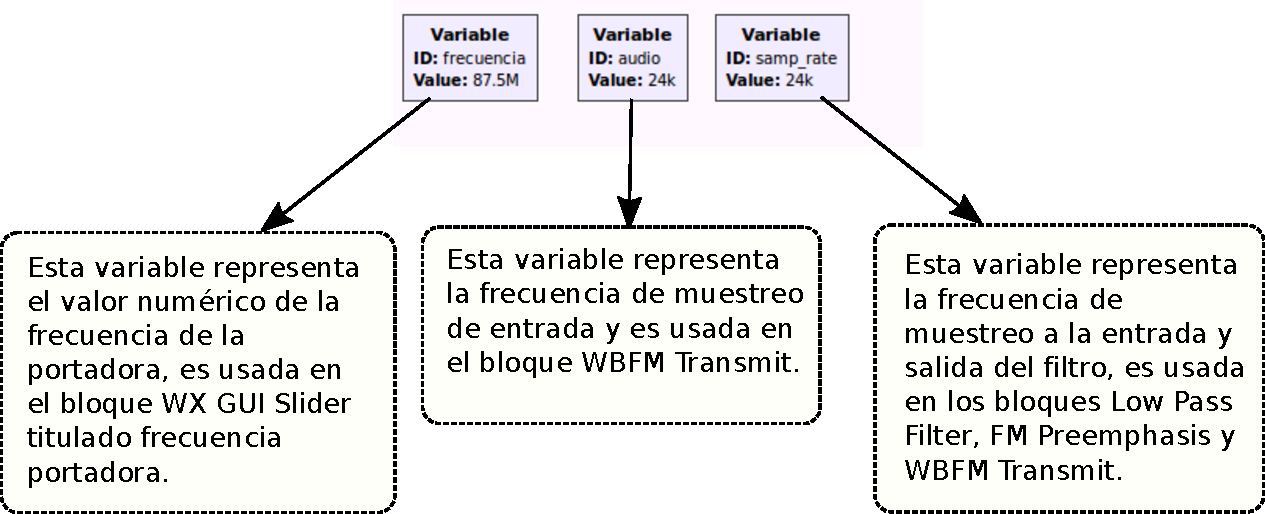
\includegraphics[width=\textwidth]{parte3/lab11/pdf/lab11_2.pdf}
\end{figure}

En este transmisor la fuente es un archivo de audio en formato WAV muestreado a 24 kHz.


\end{frame}
%---------------------------------

\begin{frame}{Transmisor FM Monofónico}

\begin{figure}[H]
\centering
\vspace{-3mm}
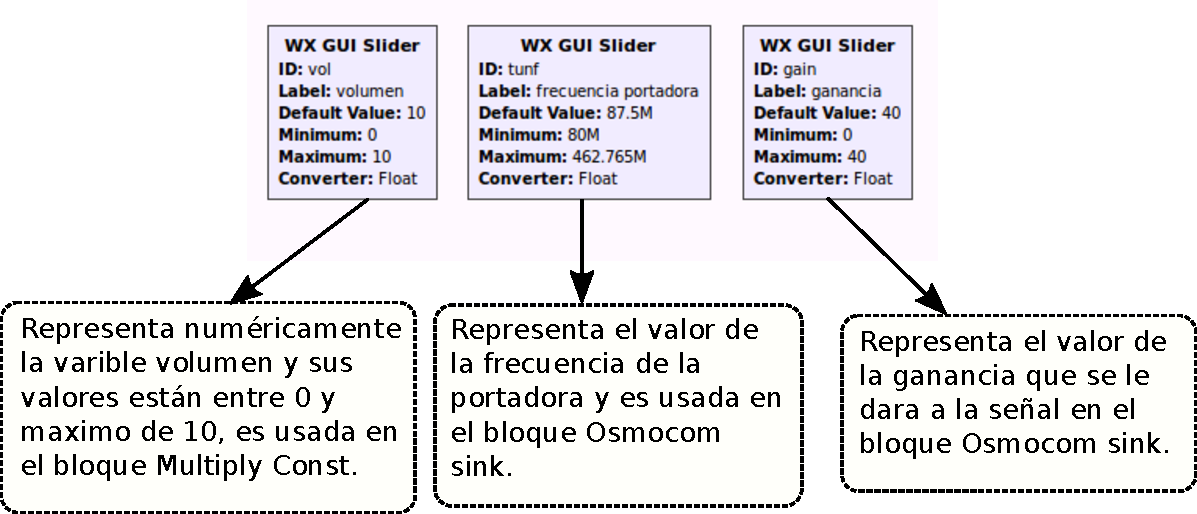
\includegraphics[width=\textwidth]{parte3/lab11/pdf/lab11_3.pdf}
\end{figure}

\end{frame}
%---------------------------------

\begin{frame}{Transmisor FM Monofónico}

\begin{figure}[H]
\centering
\vspace{-3mm}
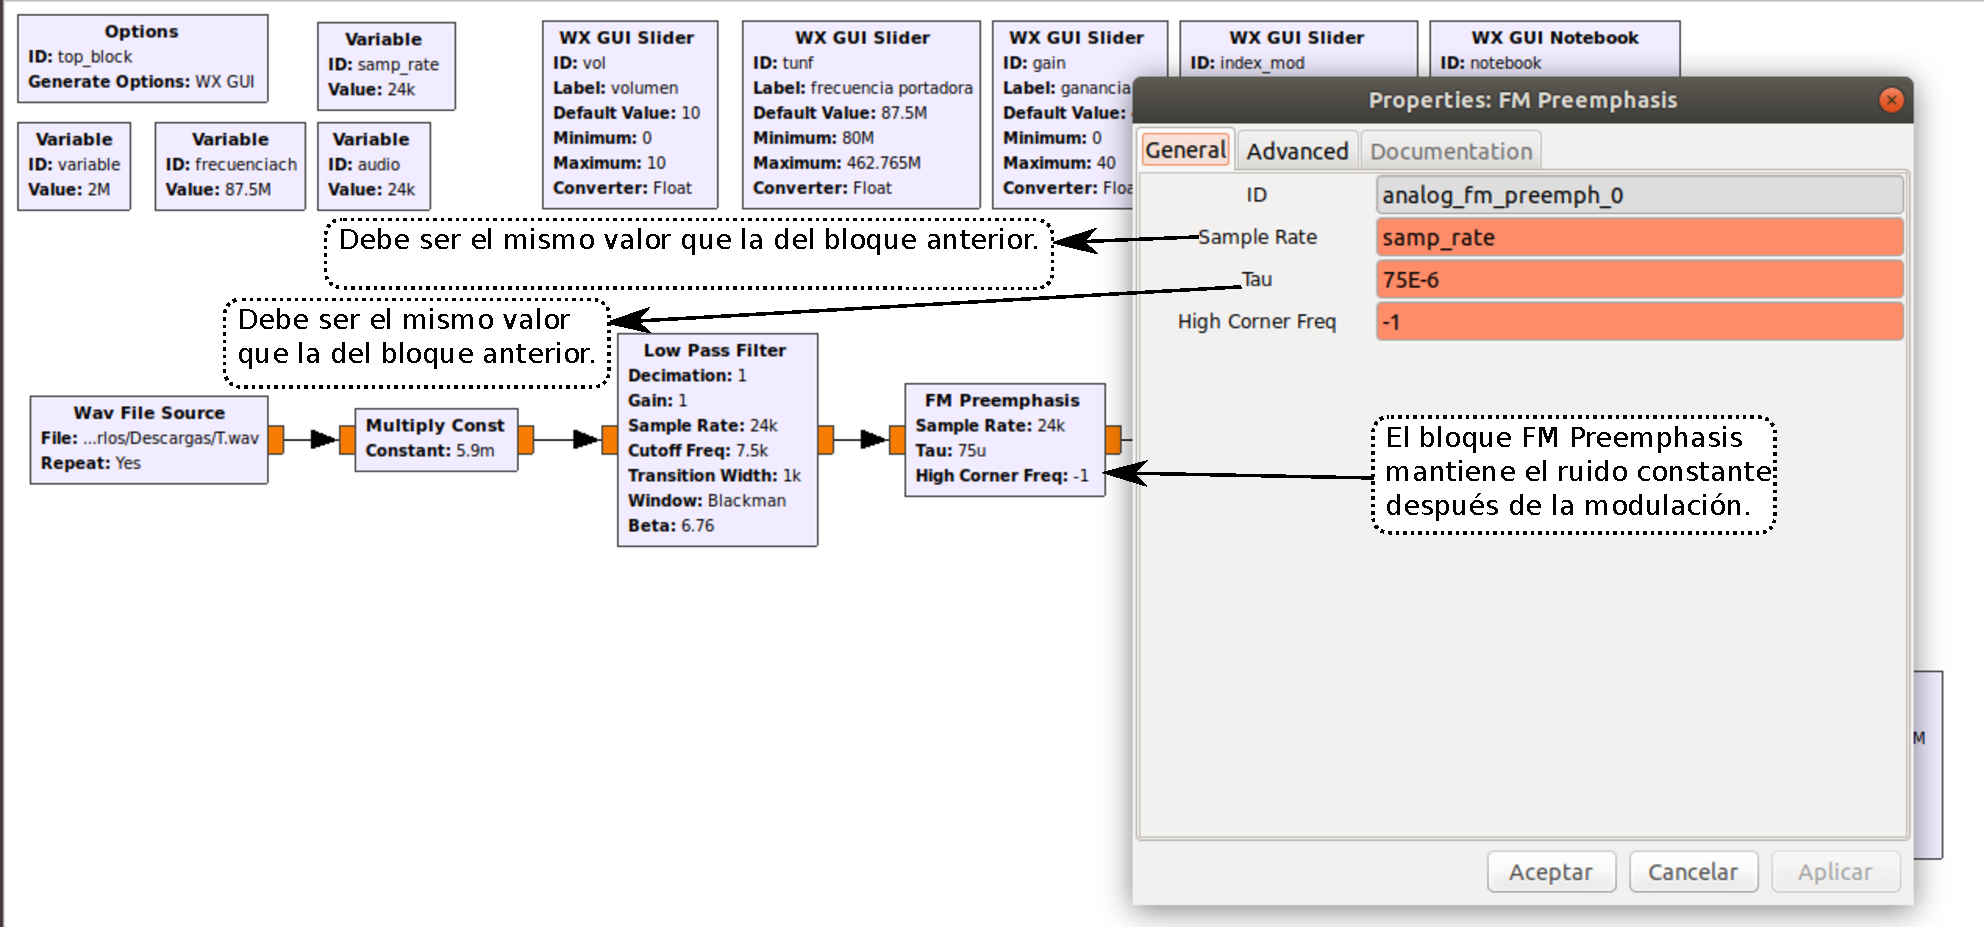
\includegraphics[width=\textwidth]{parte3/lab11/pdf/lab11_4.pdf}
\end{figure}

\end{frame}
%---------------------------------

\begin{frame}{Transmisor FM Monofónico}

\begin{figure}[H]
\centering
\vspace{-3mm}
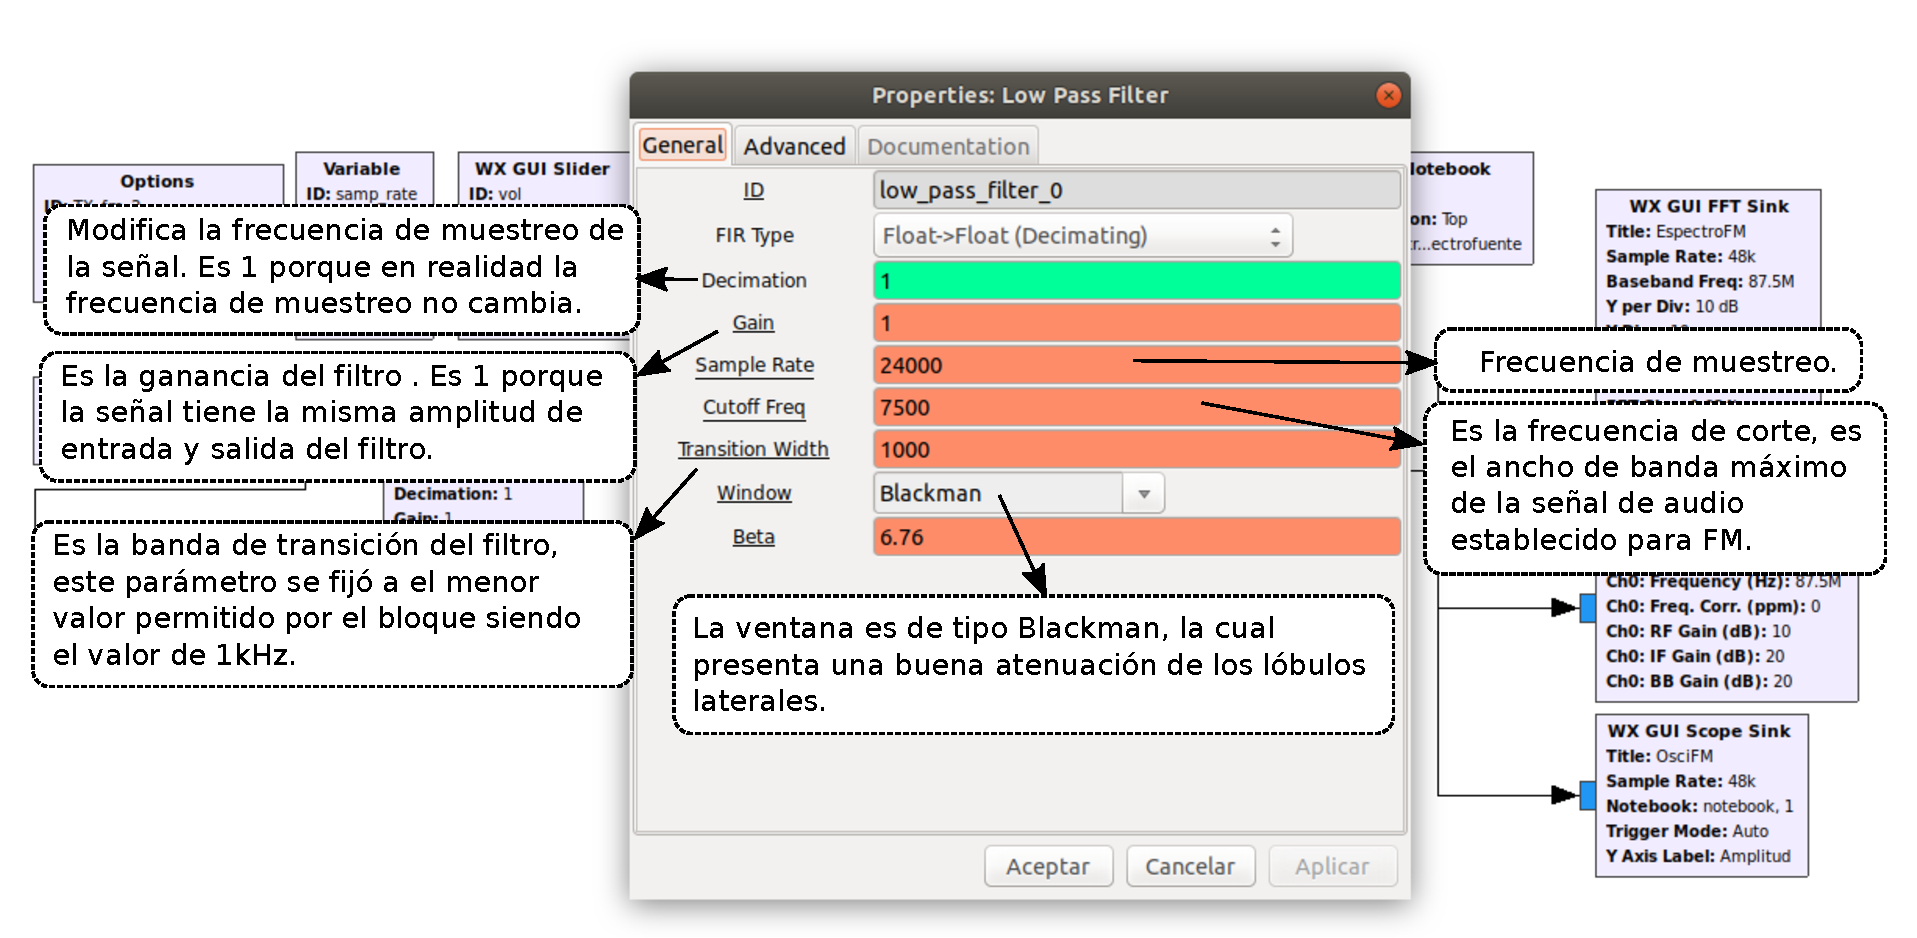
\includegraphics[width=\textwidth]{parte3/lab11/pdf/lab11_5.pdf}
\end{figure}

\end{frame}
%---------------------------------

\begin{frame}{Transmisor FM Monofónico}

\begin{figure}[H]
\centering
\vspace{-3mm}
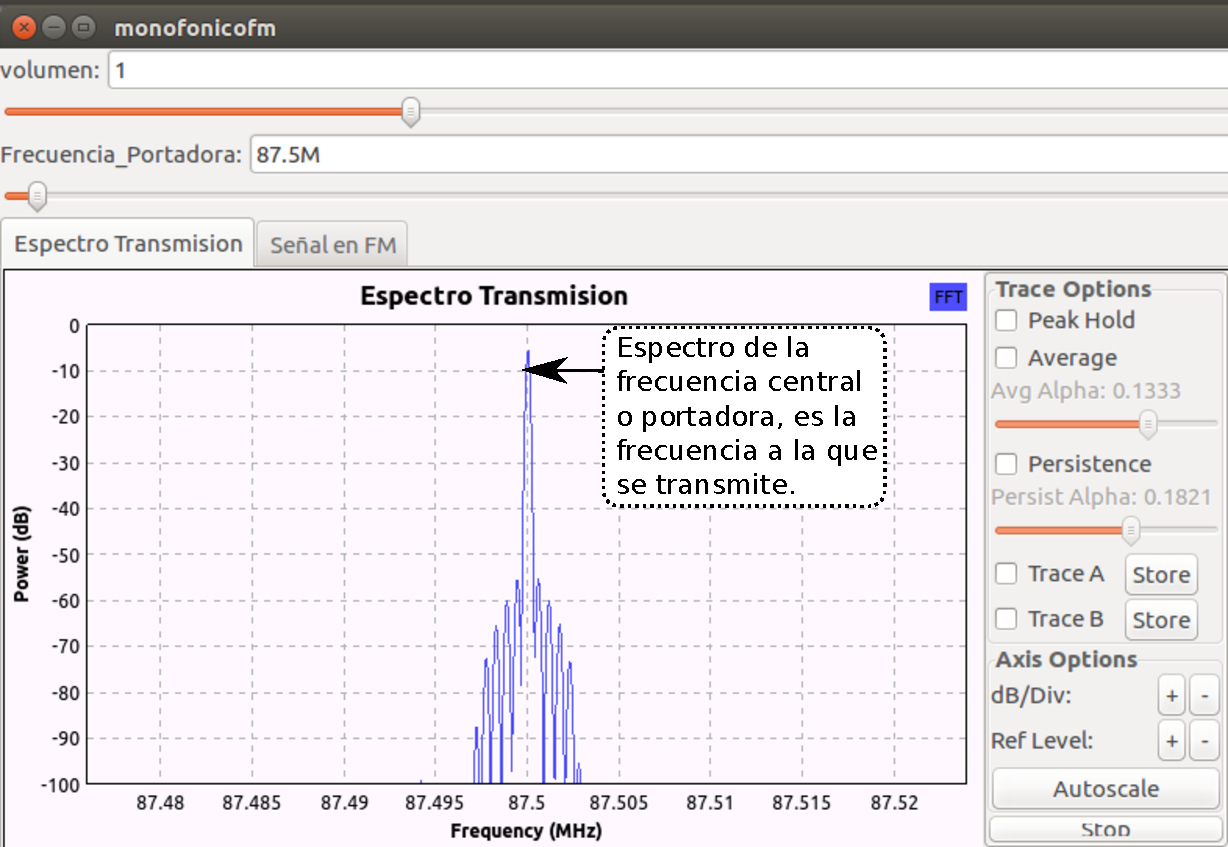
\includegraphics[width=\textwidth]{parte3/lab11/pdf/lab11_6.pdf}
\end{figure}

\end{frame}
%---------------------------------